\chapter{Disaster Plan}
\section{Outline and Scope}
This disaster management and contingency plan aims to identify risks and provide methods of mitigation. Certain network issues can be treated with automation via the setup of executables using the Intermapper network management software. If manual intervention is required, the plan employs a systematic approach, which allows problems to be treated in a sufficient timeframe, but with enough knowledge so that it can be understood and corrected properly. We have been proactive with our network design, employing the Cisco 3-layer hierarchical model to prevent issues and help with troubleshooting. Our design makes it easier to isolate a section of the network where an issue may be found, makes scaling easier and ensures we have redundancy within the network.
\section{Risks and Mitigation}
\begin{table}[H]
    \centering
    \begin{tabular}{|p{0.35\linewidth}|p{0.35\linewidth}|p{0.35\linewidth}|}
    \hline
    Risk                                                 & Potential Consequences                                                                                       & Mitigation                                                                                                                                                                                                                         \\ \hline
    Natural Disaster i.e., flooding, earthquake, tsunami & Destruction of the building or critical IT infrastructure. Loss of critical personal and manufacturing data. & Seek cloud-based computing solutions for storage of critical data in geographical locations where natural disasters are less frequent.                                                                                             \\ \hline
    Fire                                                 & Destruction or damage to critical IT infrastructure. Damage to company reputation                            & Conduct regular fire assessments, ensuring sockets are PAT tested and fire extinguishers are readily available.                                                                                                                    \\ \hline
    Power Cut                                            & Disrupt operations and potential loss of data.                                                               & Utilise the space in the underground car park for a temporary backup power supply. Ensure this power supply can handle normal business operations.                                                                                 \\ \hline
    Network Issues                                       & Loss of communications and disruption of operations.                                                         & Ensure adequate levels of redundancy are implemented into the network. Isolate network where the issue is and ensure there is enough backup equipment available to create a simple network should critical operations be required. \\ \hline
    Theft                                                & Loss of infrastructure or crucial data. Damage to reputation.                                                & Ensure IT team performs regular checks on IT devices along with trackers and encrypted hardware.                                                                                                                                   \\ \hline
    Software Issues                                      & Disruption of operations. Loss of access to data.                                                            & Perform backups regularly before updating software. If the latest versions of software cause issues, the IT team should roll back to the previous version if there is no significant vulnerability risk.                           \\ \hline
    Hardware Issues                                      & Disruption of operations. Loss of access to data.                                                            & Planned resolution methods for each network device, whether it is router, switch or computer. Isolate network where hardware issue is if needed and perform regular backups to prevent loss of data.                               \\ \hline
    Employee Lost Device                                 & Possible loss of data and/or exposure of sensitive company data.                                             & Ensure password policies are enforced on employee devices, with multi-factor authentication and encrypted hard drives.                                                                                                             \\ \hline
    \end{tabular}
    \caption{Risks and mitigations}
    \label{tab:risks_mitigations}
\end{table}

\section{Risk Assessment Matrix}

The Risk Assessment Matrix provides visual indication of how likely a risk is to occur, as well as its impact on Yotsuba Group in such an event. Mitigation methods described in Table \ref{tab:risks_mitigations} will help overcome and reduce the consequences of these risks.

\begin{figure}[H]
    \centering
    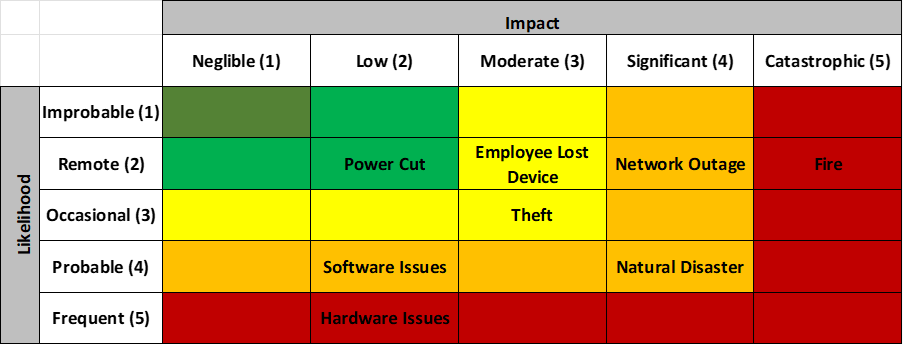
\includegraphics[width=15cm]{Figures/risk_assessment_matrix.png}
    \caption{Risk assessment matrix for Yotsuba Group}
    \label{fig: table}
\end{figure}